% !TEX options=-synctex=-1
\documentclass[a4paper,12pt]{article}
\usepackage[utf8]{inputenc}
\usepackage[T1]{fontenc}
\usepackage[french]{babel}
\usepackage{amsmath,amssymb}
\usepackage{xcolor}
\usepackage{geometry}
\usepackage{soul}
\usepackage{graphicx} % pour inclure des images

\geometry{
  a4paper,
  total={170mm,257mm},
  left=20mm,
  top=20mm,
}

\usepackage{extensionCours}

\title{TP1 - Algèbre Linéaire et Plan Complexe}
\author{Groupe 2 \\* Colin, Henri, Leïla, Loïs}

\begin{document}
\maketitle

\sectionExercice{Algèbre Linéaire}

\begin{enumerate}
    \item Résolvez le système linéaire suivant :
\[
\begin{cases}
2x + 2y = 4,\\[1mm]
3x - 8y  = -1 
\end{cases}
\]
Réponse :
\[
\begin{cases}
x = 2 - y,\\[1mm]
-11y = -7  
\end{cases}
\Rightarrow
\boxed{
\begin{cases}
x = \frac{15}{11}, \\[1mm]
y = \frac{7}{11}
\end{cases}
}
\]

    \item Dans \(\mathbb{R}^2\), considérez la base canonique \(\{e_1, e_2\}\) et une nouvelle base \(\{v_1, v_2\}\) définie par
\[
v_1 = \begin{pmatrix} 1 \\ 1 \end{pmatrix}, \quad
v_2 = \begin{pmatrix} 1 \\ -1 \end{pmatrix}.
\]
Exprimez le vecteur 
\[
w = \begin{pmatrix} 2 \\ 3 \end{pmatrix}
\]
dans la nouvelle base.
\[
\begin{cases}
\lambda_1 + \lambda_2 = 2,\\[1mm]
\lambda_1 - \lambda_2 = 3 
\end{cases}
\Rightarrow
\begin{cases}
2 \lambda_1 = 5,\\[1mm]
\lambda_2 = -\frac{1}{2} 
\end{cases}
\Rightarrow
\boxed{
w = \frac{5}{2} v_1 - \frac{1}{2} v_2
}
\]

    \item Calculez le produit scalaire des vecteurs $v_1$ et $v_2$ définis ci-dessus.

\[
v_1 \cdot v_2 = 1 \cdot 1 + 1 \cdot (-1) = 0
\Rightarrow \boxed{v_1 \cdot v_2 = 0}
\]

    \item Calculez le déterminant de la matrice :
\[
M = 
\begin{pmatrix} 
1 & 2 \\ 
2 & 3 
\end{pmatrix}
\Rightarrow
\det(M) = 1 \cdot 3 - 2 \cdot 2 = -1
\Rightarrow \boxed{\det(M) = -1}
\]
\end{enumerate}

\newpage

\sectionExercice{Fractales et Ensemble de Julia}

\subsection*{Objectif}

Ce second exercice avait pour but de visualiser l'ensemble de Julia associé à une fonction complexe de la forme :
\[
f_c(z) = z^2 + c
\]
où \(c\) est un paramètre complexe fixé et \(z\) une variable complexe. L'objectif était de générer une image montrant les zones de l'ensemble de Julia pour différentes valeurs de \(c\).

\subsection*{Démarche}

L'ensemble de Julia est généré en parcourant chaque pixel de l'écran, et en l'associant à un point \(z_0\) du plan complexe. Pour chaque \(z_0\), on évalue la suite :
\[
z_{n+1} = z_n^2 + c
\]
jusqu'à ce que la norme \(|z_n|\) dépasse 2, ou qu’un nombre maximal d’itérations soit atteint. Si la suite diverge, on note le nombre d’itérations nécessaires.

Le programme se base sur les étapes suivantes :

\begin{itemize}
    \item Chaque pixel \((x, y)\) est converti en un nombre complexe \(z_0\) en transformant les coordonnées de l'écran vers le plan complexe.
    \item Une fonction \texttt{julia} retourne le nombre d’itérations effectuées avant divergence (ou la valeur maximale si la suite reste bornée).
    \item Ce nombre est utilisé pour colorer le pixel : noir si la suite est bornée, ou une couleur dépendant de la vitesse de divergence, choisie dans le spectre HSV (teinte variant en fonction du nombre d’itérations).
\end{itemize}

\subsection*{Implémentation et Utilisation}

Le code de cette visualisation est contenu dans le fichier \texttt{julia\_viewer.py}, situé dans le dossier \texttt{geometry\_engine\_executables}.

Pour exécuter ce programme dans \textbf{Sublime Text}, il suffit de presser \texttt{Ctrl + Shift + B}, puis de sélectionner la commande \texttt{run\_julia\_viewer}.

Il est également possible de lancer le programme directement depuis un terminal.

\subsection*{Conclusion}

Ce TP nous a permis d’aborder la construction des ensembles de Julia sous un angle mathématique et algorithmique. En explorant le comportement de suites complexes selon différents paramètres, nous avons observé comment des règles simples peuvent générer des structures complexes. Ce travail met en lumière l’interaction entre analyse complexe, calcul numérique et représentation graphique, et illustre l’intérêt de la visualisation pour mieux comprendre certains phénomènes mathématiques.

\clearpage

\subsection*{Annexe – Exemple de rendu}

Voici un exemple de visualisation générée pour la valeur \( c = -0.7 + 0.27015i \) :

\begin{figure}[h]
    \centering
    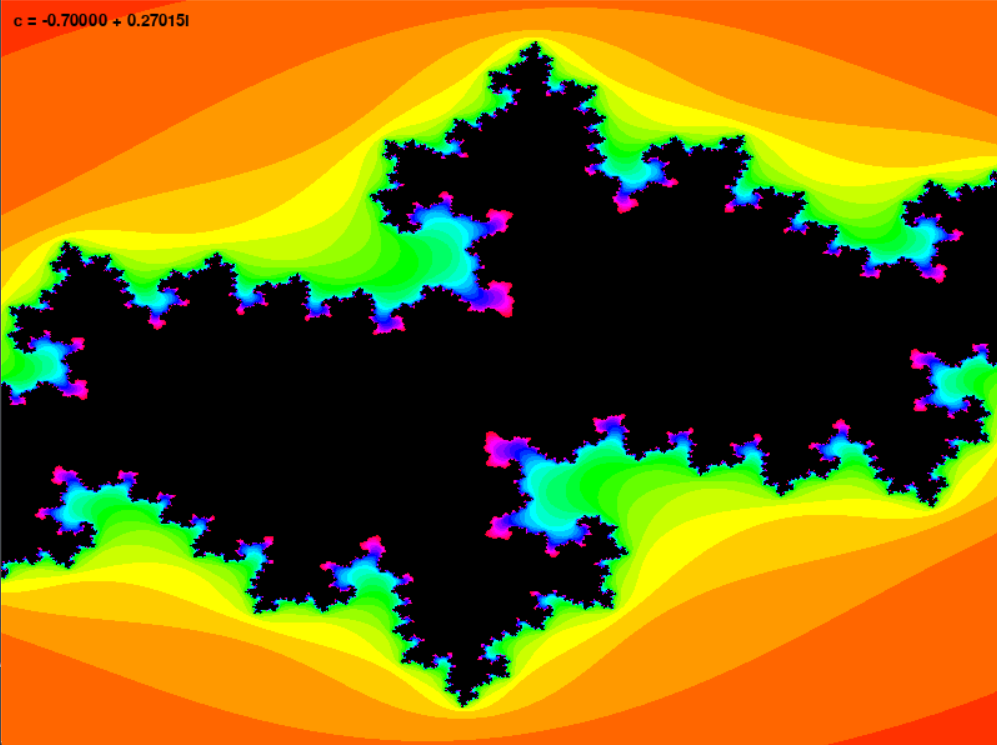
\includegraphics[width=0.8\textwidth]{julia_set_example.png}
    \caption{Ensemble de Julia pour \( c = -0.7 + 0.27015i \).}
    \label{fig:julia_set}
\end{figure}

\end{document}
